\documentclass[
% handout,
center,
% aspectratio=169
]{beamer}

\usepackage[utf8]{inputenc}
\usepackage[english]{babel}
\usepackage{cite}
\usepackage{amsmath,amssymb,amsfonts}
\usepackage[linesnumbered,ruled,vlined]{algorithm2e}
\usepackage[noabbrev,capitalize]{cleveref}
\usepackage{array, booktabs, makecell}
\usepackage{graphicx}
\usepackage{textcomp}
\usepackage{xcolor}
\usepackage{caption}
\usepackage{subcaption}
\usepackage{diagbox}
\usepackage{tikz}
\usepackage{soul}
\DontPrintSemicolon

\title[Huffman Coding]{\textsc{Huffman Coding}}
\author[Bozzo - Yin]{Francesco Bozzo \and Michele Yin}
\institute[UniTN]{University of Trento}
\date{December 15, 2022}

% \logo{\includegraphics[height=1.5cm]{logo.png}}
%\usetheme{Madrid}
\definecolor{links}{HTML}{54489a}
\hypersetup{colorlinks,linkcolor=,urlcolor=links}
\usetheme{metropolis}
\setbeamercolor{background canvas}{bg=white}

\begin{document}

\begin{frame}
\titlepage
\end{frame}

% table of contents
% \AtBeginSection[]
% {
%     \begin{frame}{Table of Contents}
%         \begin{columns}[t]
%             \column{.45\textwidth}
%             \tableofcontents[sections=1-2, currentsection]

%             \column{.45\textwidth}
%             \tableofcontents[sections=3-5, currentsection]
%         \end{columns}
%     \end{frame}
% }

\section{Introduction}

\begin{frame}{Introduction}
    Table of contents
    \begin{itemize}
        \item The Huffman Coding Algorithm
        \item Serial Implementation
        \item Parallel Implementation
        \item Performance Evaluation and Benchmarks
        \item Q\&A
    \end{itemize}
\end{frame}

\begin{frame}{The Huffman Coding Algorithm}
    Huffman Coding is a \textbf{lossless data compression} algorithm  designed to find a more convenient bit representation to store data through variable-length sequences of bits defined as \emph{alphabet}.
    \begin{table}[]
        \centering
        \begin{tabular}{lll}
            \toprule
            ASCII character & Byte encoding & Huffman encoding \\
            \midrule
             a &  01100001 & 00 \\
             b &  01100010 & 010 \\
             c &  01100011 & 011 \\
             d &  01100100 & 10 \\
             e &  01100100 & 11 \\
             \bottomrule
        \end{tabular}
        \caption{Example of Huffman alphabet for 5 letters}
        \label{tab:my_label}
    \end{table}
\end{frame}

\begin{frame}{Frequency-based Encoding}
    The Huffman code for each character is decided by the occurrences of that character in the text using a \textbf{greedy} procedure:
    \begin{itemize}
        \item more frequent -> less bits
        \item less frequent -> more bits
    \end{itemize}
\end{frame}

\begin{frame}{Optimal Prefix Code}
    Even if the the Huffman algorithm is based on a greedy approach, it is able to generate an \textbf{optimal prefix code} in space efficiency.
\end{frame}

\section{Serial Version}

\begin{frame}{Serial Version}
    The Huffman Compression Algorithm is composed by four phases:
    \begin{enumerate}
        \item Count the byte frequencies
        \item Build the Huffman tree using the frequencies
        \item Generate the Huffman alphabet by visiting the Huffman tree by using a DFS algorithm
        \item Data encoding using the Huffman alphabet
    \end{enumerate}
\end{frame}

\begin{frame}{Build the Huffman Tree}
    \centering
    \scalebox{.8}{
        \begin{algorithm}[H]
            \caption{Build the Huffman tree}\label{alg:buildtree}
            \SetKwData{Q}{Q}\SetKwData{z1}{z1}\SetKwData{z2}{z2}\SetKwData{z}{z}
            \SetKwFunction{insert}{insert}\SetKwFunction{deleteMin}{deleteMin}
            \SetKwInOut{Input}{input}\SetKwInOut{Output}{output}
            \SetKwFor{}{}{}{}
            // Populate the min priority queue with characters and their frequencies\;
            \For{\(i=1\) \KwTo \(n-1\)}{
                Q.insert(f[i], Tree(f[i], c[i]))\;
            }
            // Repeat until the queue has only a single element left\;
            \For{\(i=1\) \KwTo \(n-1\)}{
                // Get the two least frequent nodes\;
                z1, z2 = Q.deleteMin(), Q.deleteMin()\;
                // Create and insert inner tree node into the queue\;
                z = Tree(z1.f + z2.f, null)\;
                z.left, z.right = z1, z2\;
                Q.insert(z.f, z)\;
            }
            // The last element in the queue is the root of the Huffman tree\;
            \Return{Q.deleteMin()}\;
        \end{algorithm}
    }
\end{frame}

\begin{frame}{Get the Huffman Alphabet from the Tree}
    Make a DFS visit of the Tree from root to leaves
    \begin{center}
        \begin{figure}[h!]
            \centering
            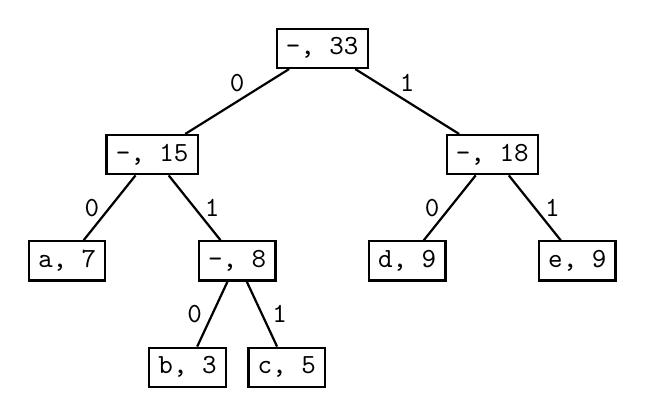
\begin{tikzpicture}
                [
                    level distance=1.5cm,
                    level 1/.style={sibling distance=4.8cm},
                    level 2/.style={sibling distance=2.4cm},
                    level 3/.style={sibling distance=1.4cm},
                    thick,
                    font=\ttfamily\bfseries, scale=0.9
                ]
                \tikzset{
                    treenode/.style = {rectangle, draw=black, align=center,minimum width=0.75cm},
                    edgestyleL/.style = {midway,left,draw=none},
                    edgestyleR/.style = {midway,right,draw=none}
                }
                \node [treenode] (T) {-, 33}
                child { node[treenode] (L) {-, 15}
                        child { node[treenode] (LL) {a, 7} edge from parent node[edgestyleL] {0} }
                        child { node[treenode] (LR) {-, 8}
                                child { node[treenode] (LRL) {b, 3} edge from parent node[edgestyleL] {0} }
                                child { node[treenode] (LRR) {c, 5} edge from parent node[edgestyleR] {1} }
                                edge from parent node[edgestyleR] {1}
                            }
                        edge from parent node[edgestyleL,above] {0}
                    }
                child { node[treenode] (R) {-, 18}
                        child { node[treenode] {d, 9} edge from parent node[edgestyleL] {0}}
                        child { node[treenode] {e, 9} edge from parent node[edgestyleR] {1}}
                        edge from parent node[edgestyleR,above] {1}
                    }
                ;
            \end{tikzpicture}
            \caption{An example of Huffman tree.}
            \label{fig:tree}
        \end{figure}
    \end{center}
\end{frame}



\section{Parallelization}
\begin{frame}{\st{Serial} Parallel Version}
    The Huffman Compression Algorithm is composed by four phases:
    \begin{enumerate}
        \item \textbf{Count} the byte frequencies
        \item Build the Huffman tree using the frequencies
        \item Generate the Huffman alphabet by visiting the Huffman tree by using a DFS algorithm
        \item \textbf{Data encoding} using the Huffman alphabet
    \end{enumerate}
    Step 1 and 4 are the most expensive and easiest to parallelize
\end{frame}
\begin{frame}{Parallelization}
    \begin{itemize}
        \item Multiple \textbf{processes} should handle separate files.
        \item Multiple \textbf{threads} of the same process should work on different chunks of the same file in parallel.
    \end{itemize}
\end{frame}
\begin{frame}{Reasoning}
    \begin{itemize}
        \item In most operating systems a file is a resource that the OS gives to a single process to avoid I/O race conditions.
        \item Because threads of the same process share the address space, we can avoid the expensive data transfer across processes.
    \end{itemize}
\end{frame}

\begin{frame}{Multithreading}
    Given $m$ threads:

    \begin{enumerate}
        \item A file is divided into $c$ \emph{chunks}, usually $m < c$ 
        \item Until all chunks are not processed:
        \begin{enumerate}
            \item A single thread reads $m$ chunks and stores them in a shared memory space
            \item Each thread works on its own assigned chunk
            \item A single thread writes the processed chunks on the disk
        \end{enumerate}
    \end{enumerate}
\end{frame}

\begin{frame}{Architecture}
    \begin{figure}
        \centering
        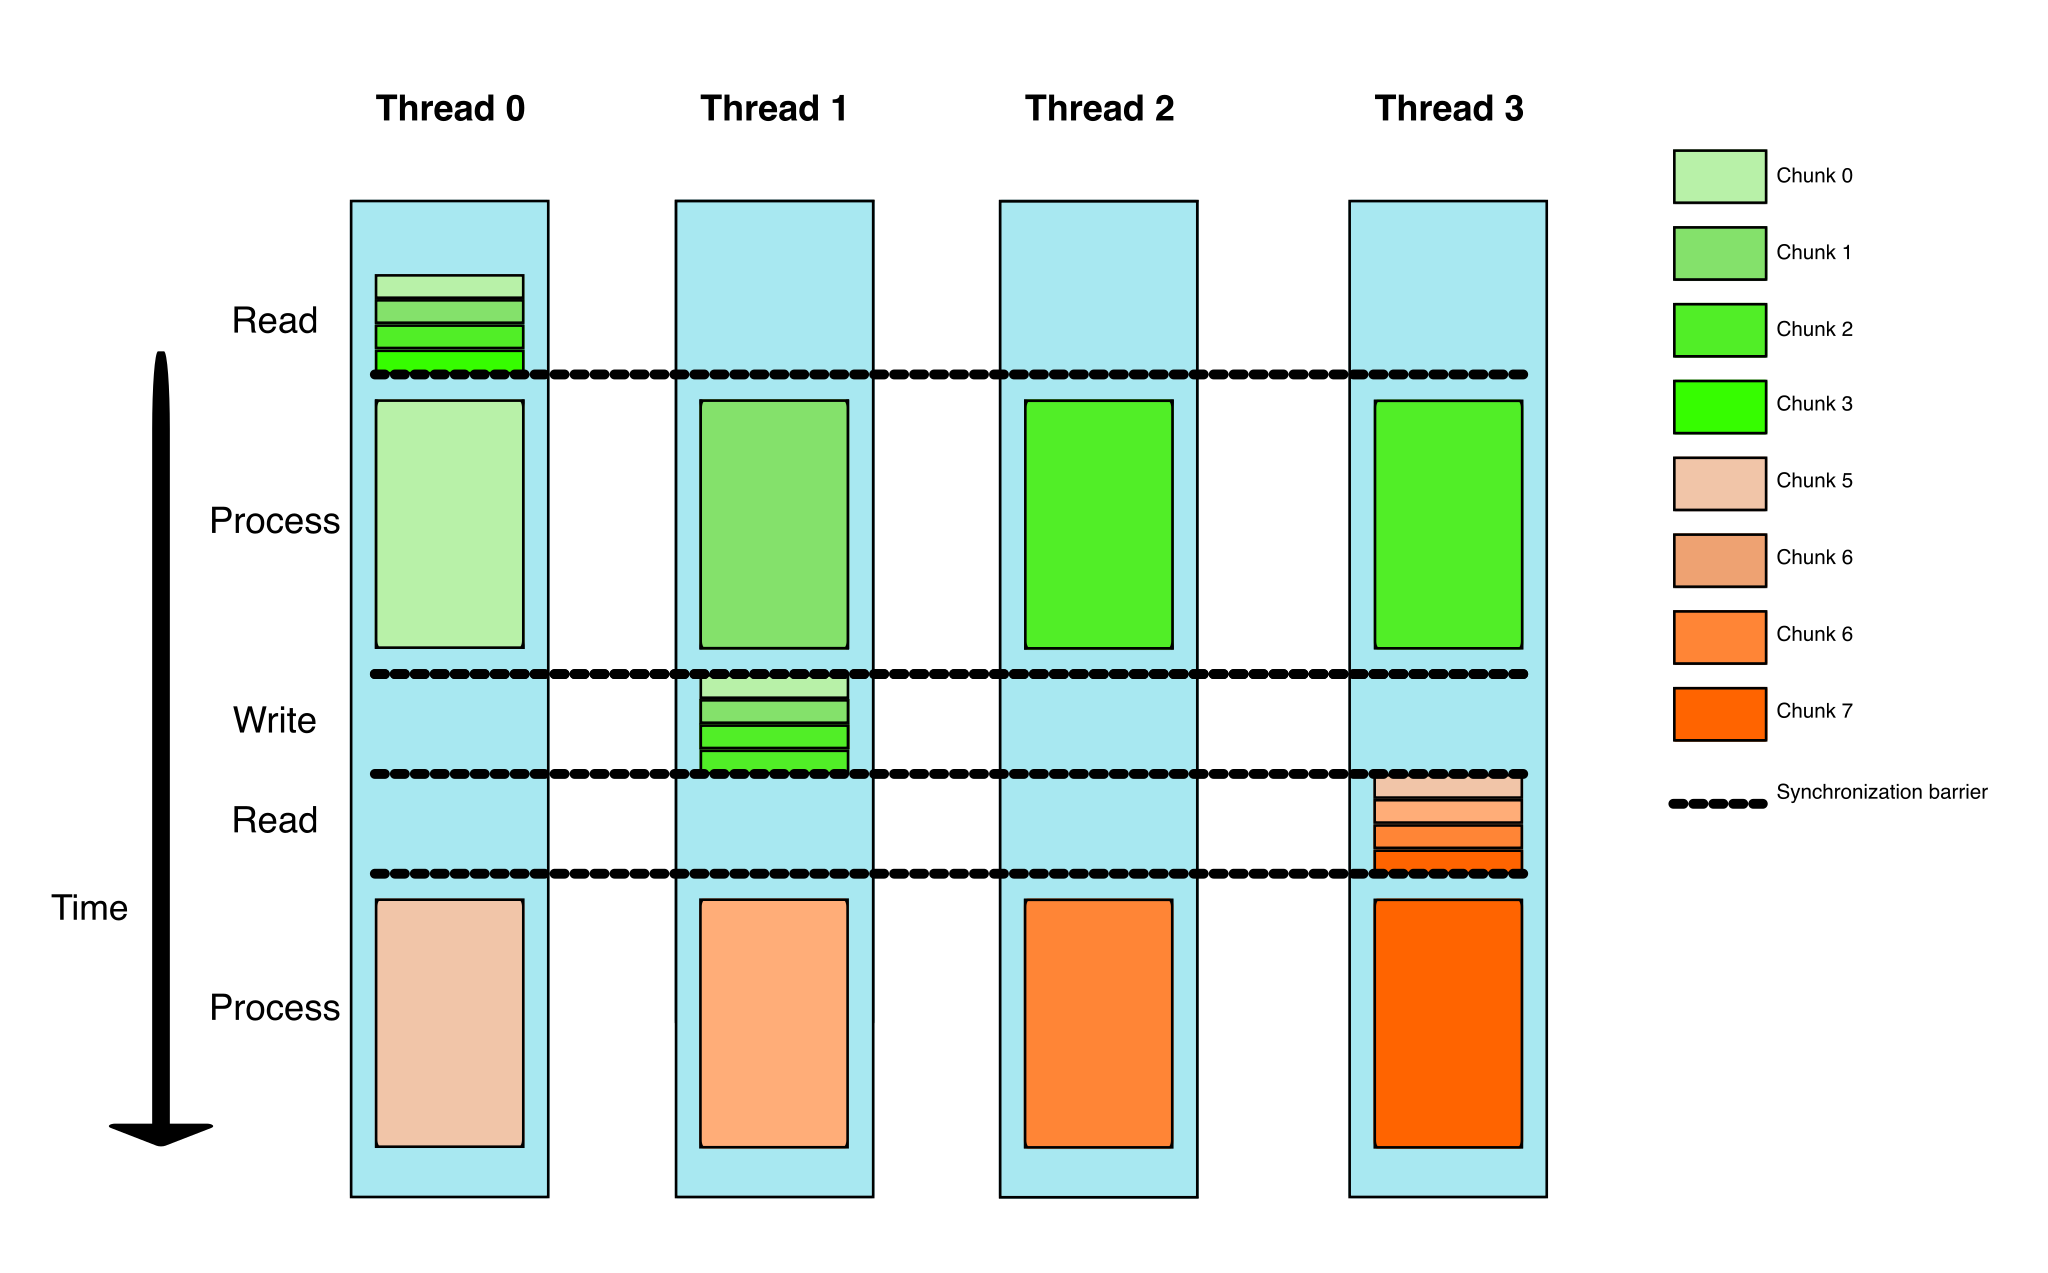
\includegraphics[width=\linewidth]{../imgs/threading}
        \caption{Simple schema for processing a single file with multiple threads.}
        \label{fig:threading}
    \end{figure}
\end{frame}
  \begin{frame}{Multiprocessing}
    \begin{itemize}
        \item Rank 0 gathers all files in the input folder
        \item Reads their size
        \item Distributes to other processes files, balancing the load using a min priority Q
        \item Each process work on its own queue of jobs 
    \end{itemize}
\end{frame}
    \begin{frame}{Multiprocess Architecture}
    \begin{figure}
        \centering
        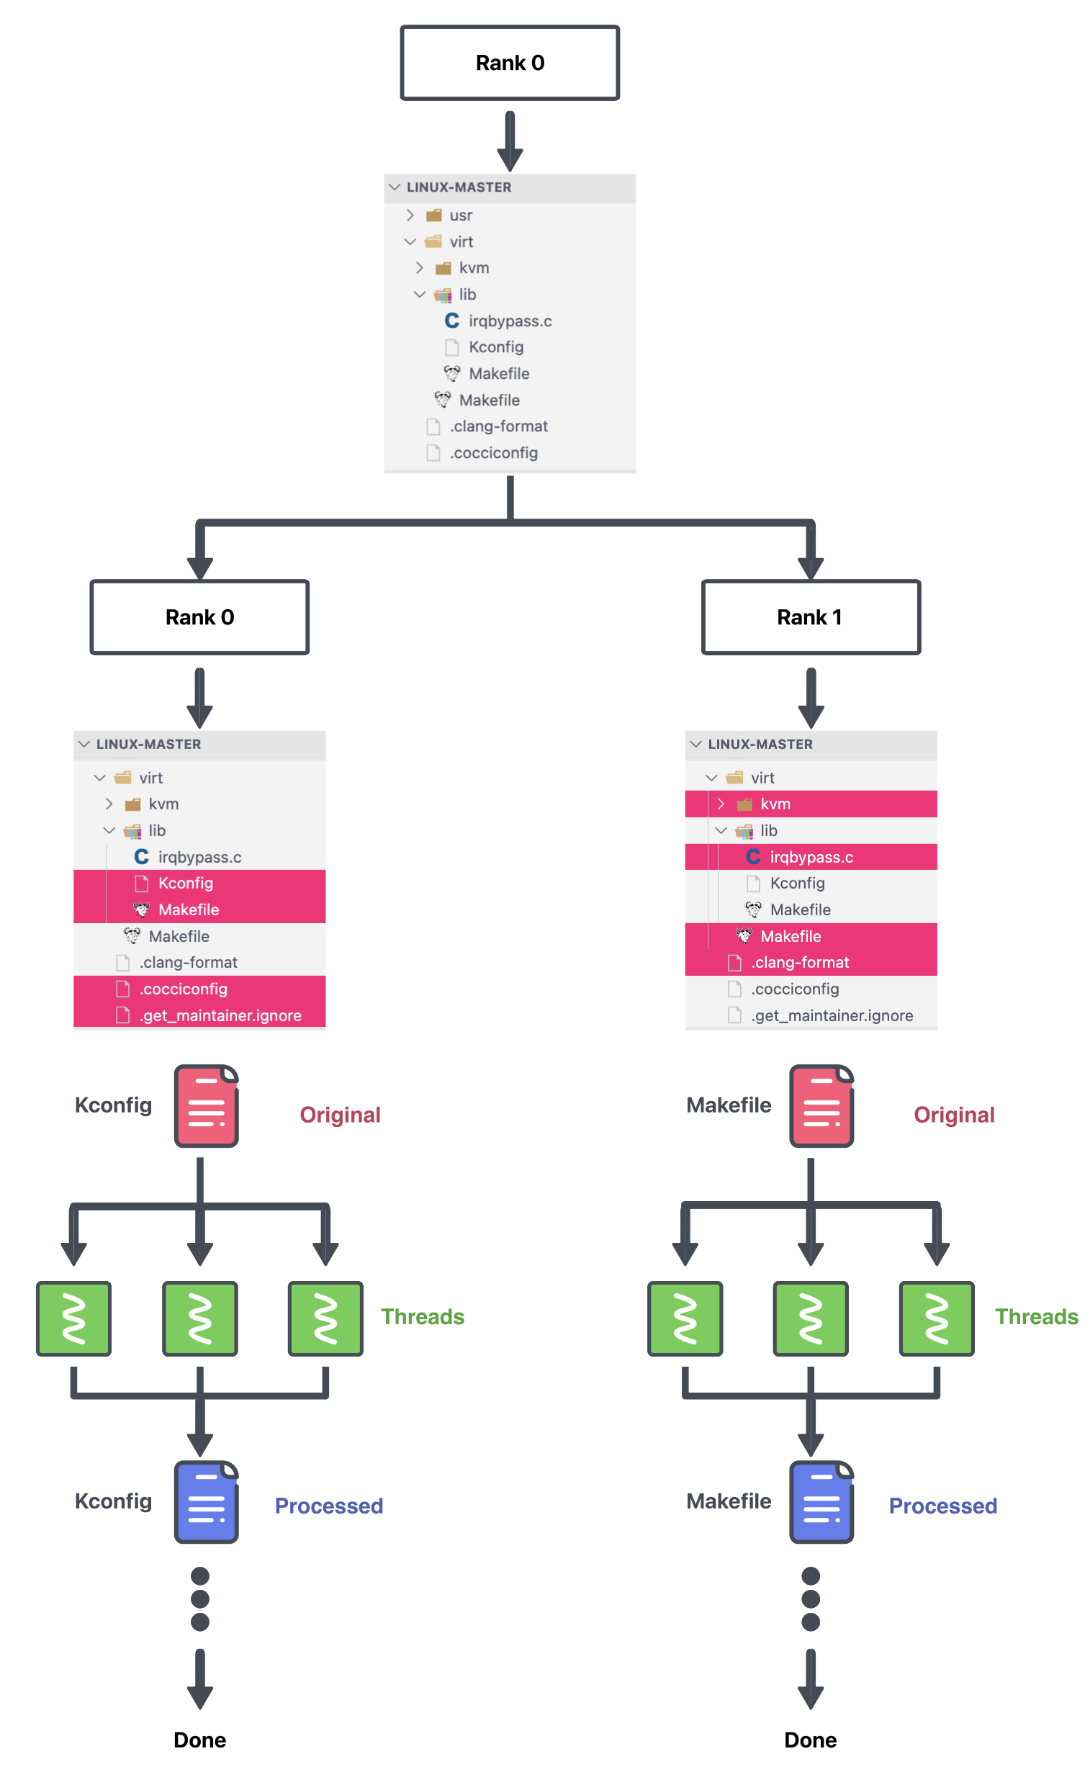
\includegraphics[width=0.40\textwidth]{../imgs/overall flow schema.png}
        \caption{Simple overall schema}
        \label{fig:threading}
    \end{figure}
\end{frame}
\begin{frame}{Implementation notes}
    \begin{itemize}
        \item 1 byte as alphabet. More bytes results in less collisions and therefore less efficiency
        \item 4096 B as chunk size, because it is the standard linux page size
        %\item I/O is not real I/O, but is a request to the OS to do the I/O
    \end{itemize}
\end{frame} 

\begin{frame}{Alternative Architecture (with Locks)}
    \begin{figure}
        \centering
        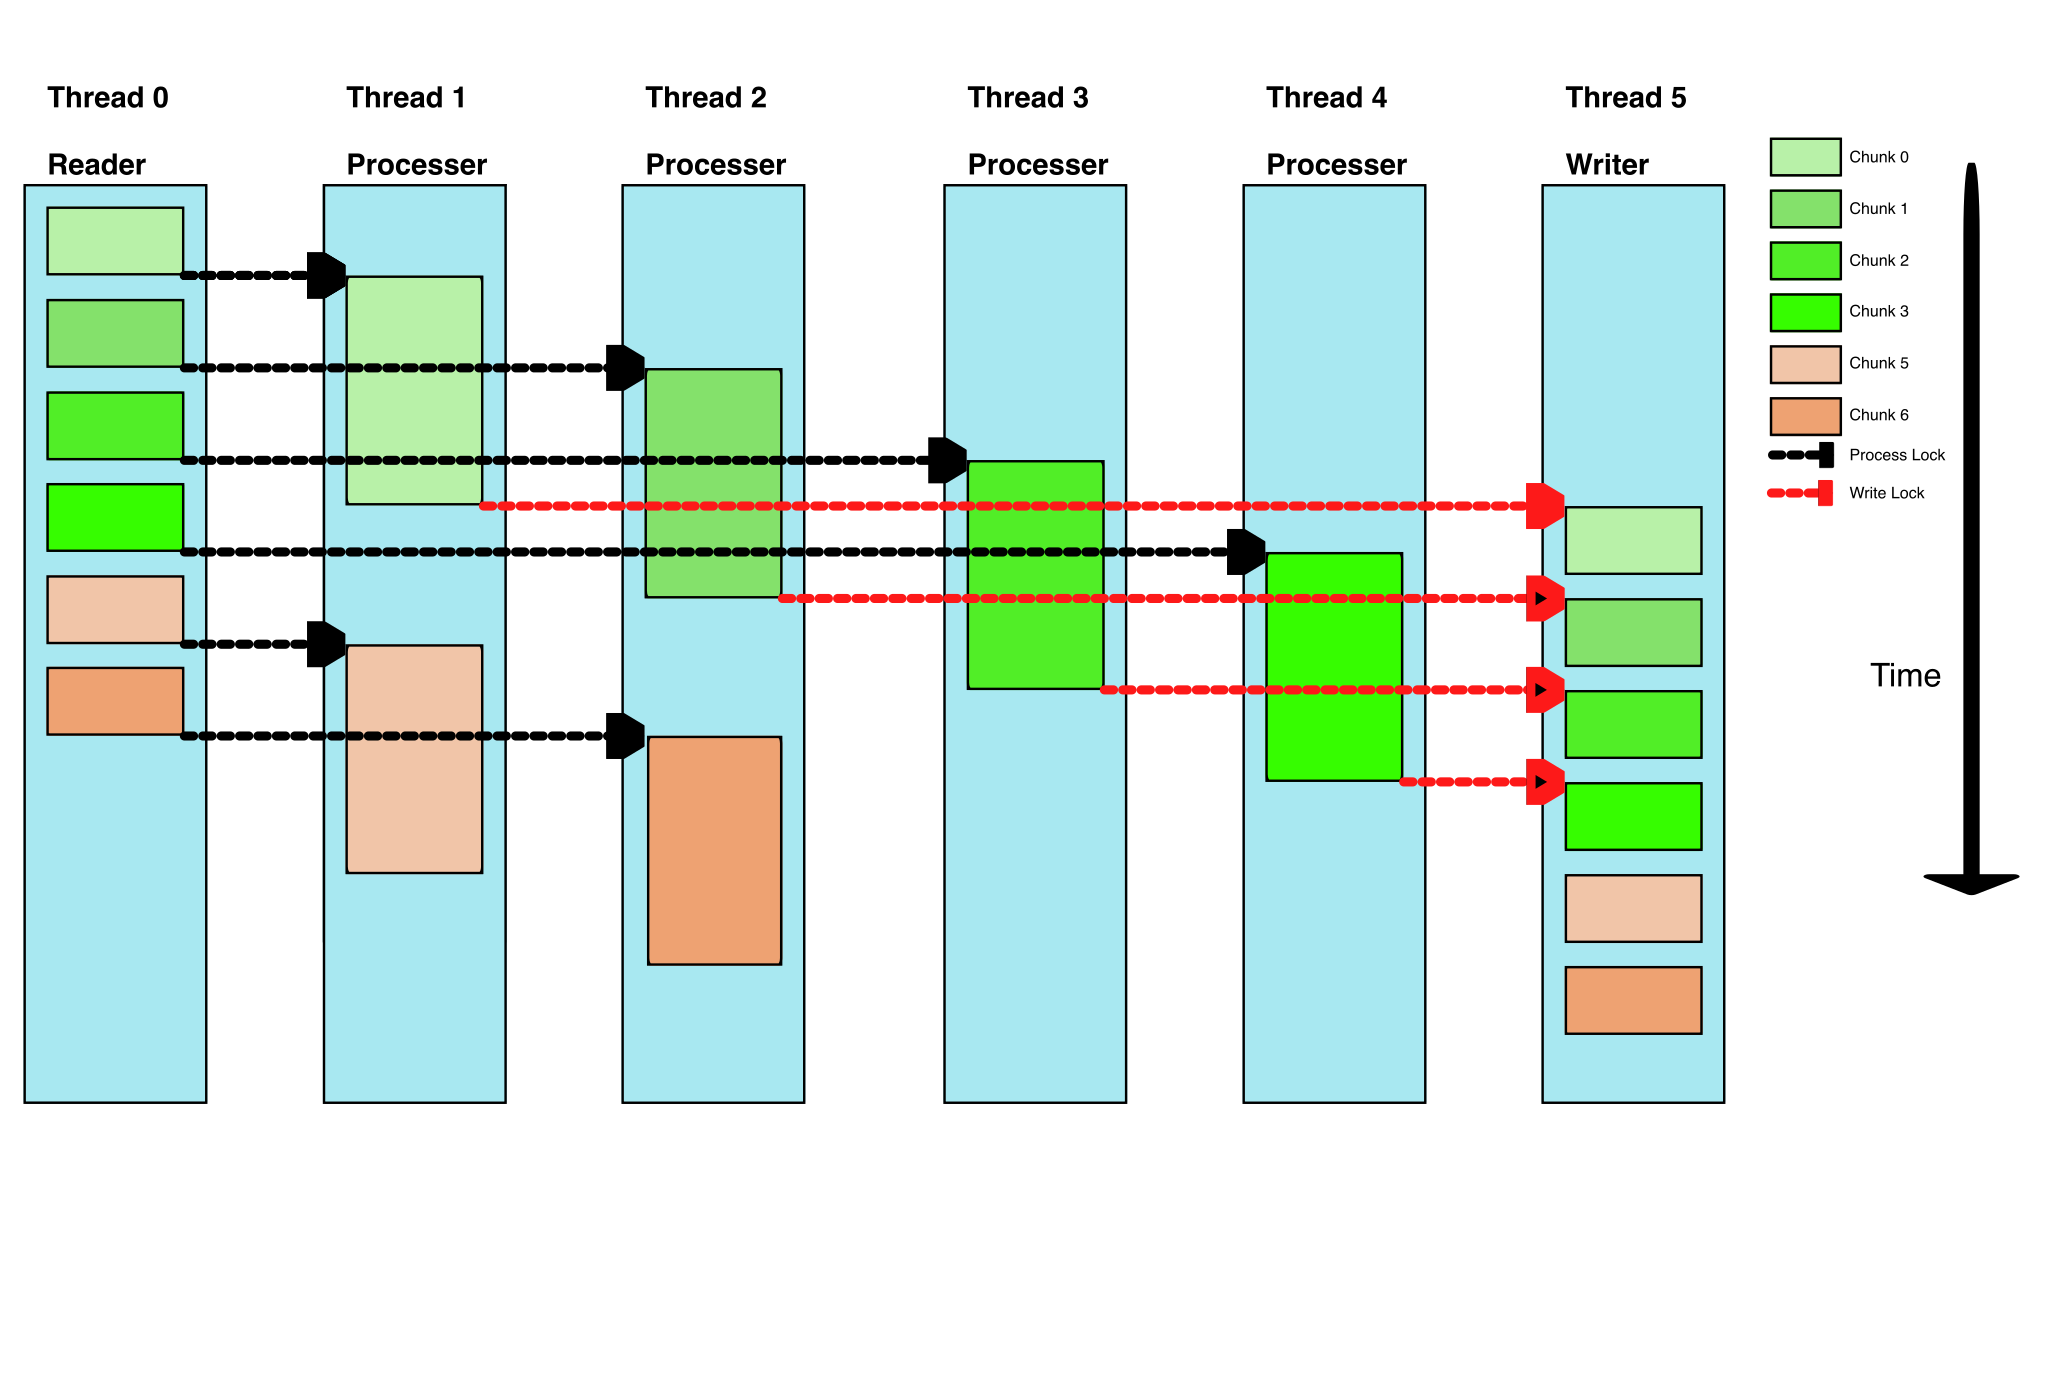
\includegraphics[width=\linewidth]{../imgs/dedicated IO threads}
        \caption{Simple schema for processing a multiple files.}
        \label{fig:threading}
    \end{figure}
\end{frame}

\section{Performance and Results}
% \begin{frame}{Results}
%     \begin{columns}
%         \column{0.5\textwidth}
%             \begin{figure}
%                 \centering
%                 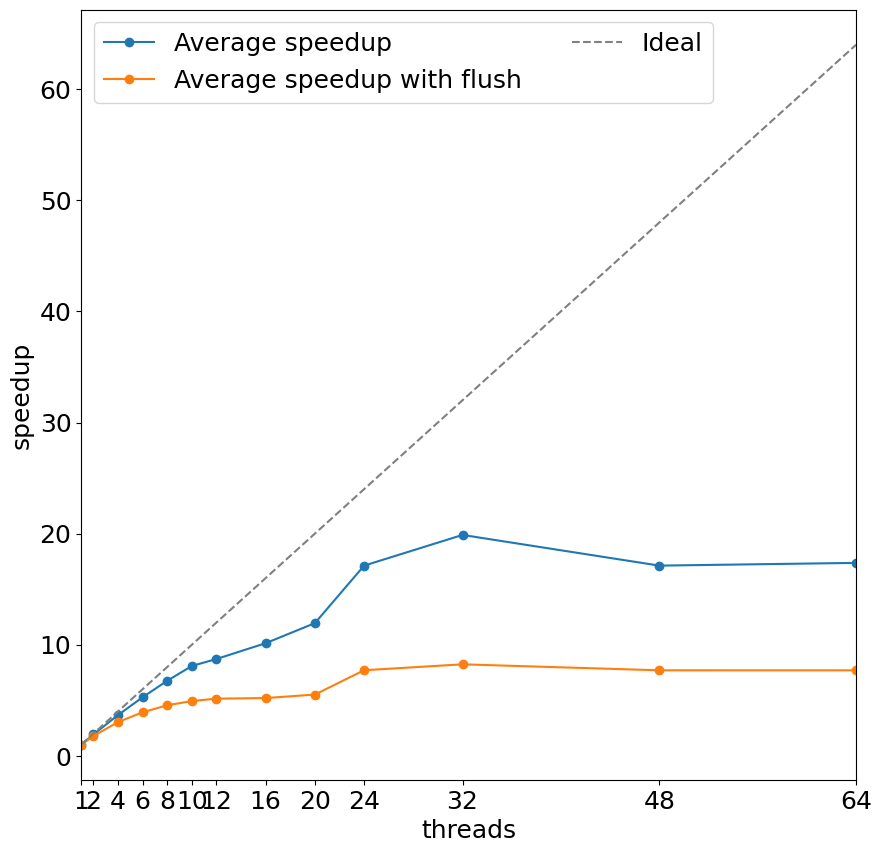
\includegraphics[width=\textwidth]{imgs/encoding average speedup.png}
%                 \caption{Encoding speedup vs flush}
%                 \label{fig:encoding-speedup-vs-flush}
%             \end{figure}
%         \column{0.5\textwidth}
%             \begin{figure}
%                 \centering
%                 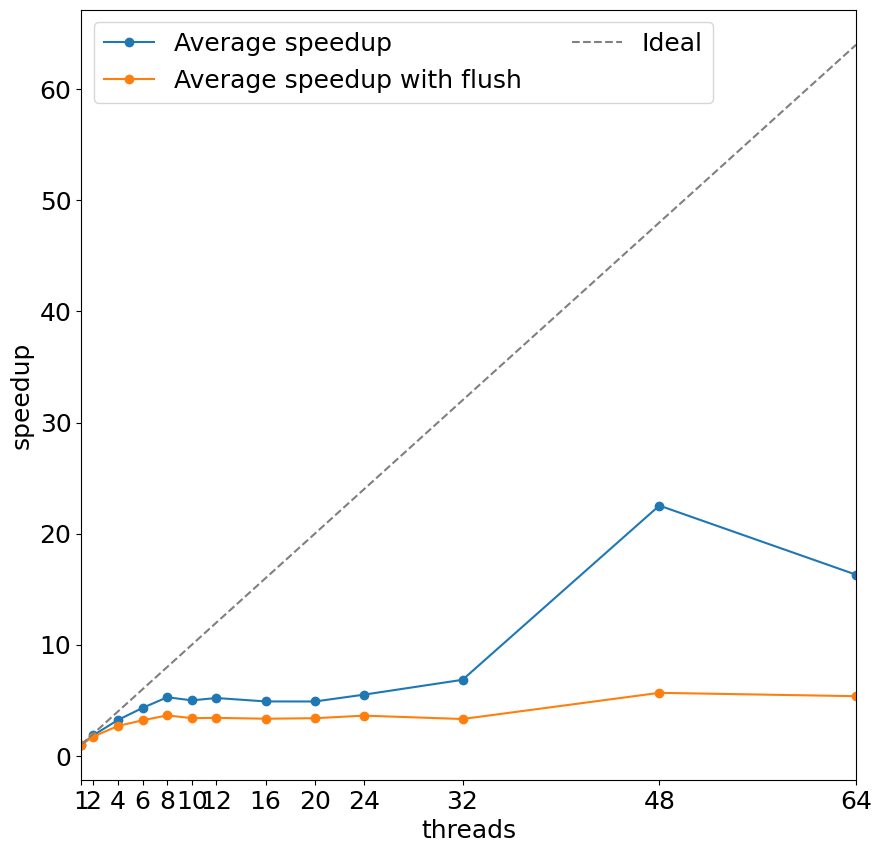
\includegraphics[width=\textwidth]{imgs/decoding average speedup.png}
%                 \caption{Decoding speedup vs flush}
%                 \label{fig:decoding-speedup-vs-flush}
%             \end{figure}
%     \end{columns}
% \end{frame}

\begin{frame}{Results - Encoding}
    \begin{columns}
        \column{0.5\textwidth}
            \begin{figure}
                \centering
                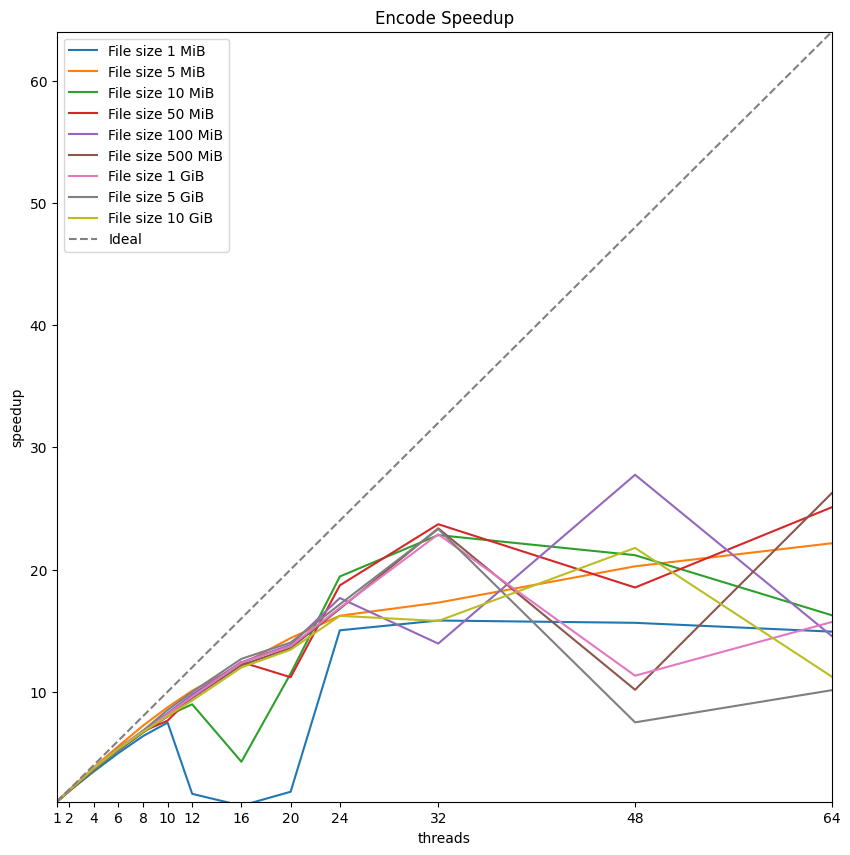
\includegraphics[width=\textwidth]{imgs/encoding speedup.png}
                \caption{Encoding speedup}
                \label{fig:encoding-speedup}
            \end{figure}
        \column{0.5\textwidth}
            \begin{figure}
                \centering
                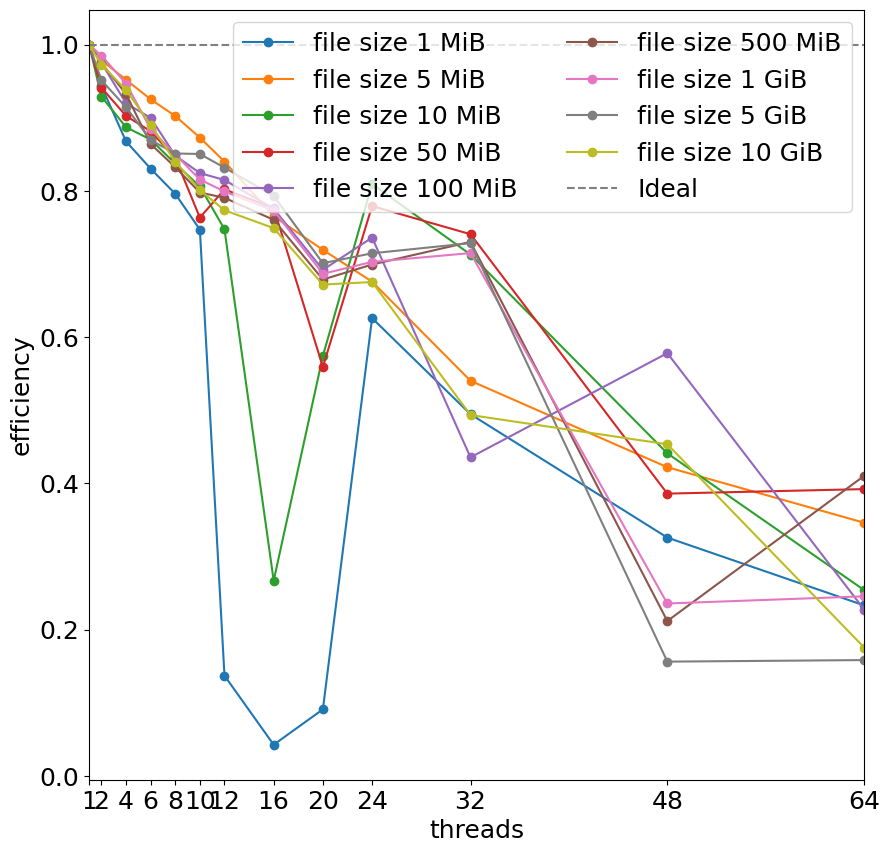
\includegraphics[width=\textwidth]{imgs/encode efficiency.png}
                \caption{Encoding efficiency}
                \label{fig:encoding-efficiency}
            \end{figure}
    \end{columns}
\end{frame}
\begin{frame}{Results - Decoding}
    \begin{columns}
        \column{0.5\textwidth}
            \begin{figure}
                \centering
                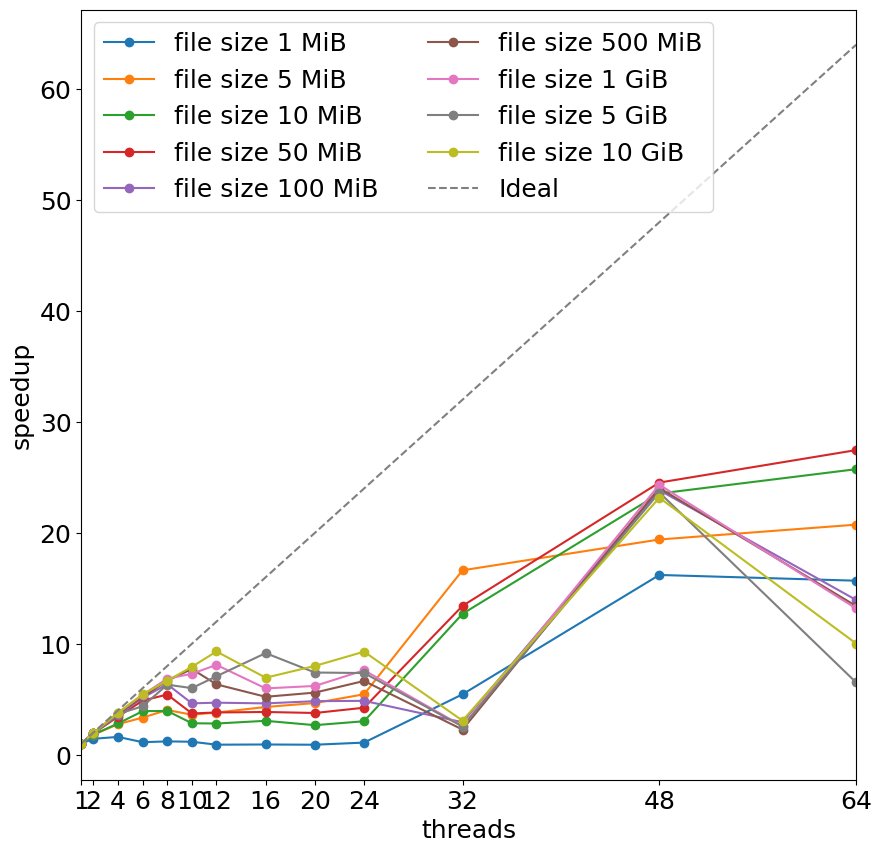
\includegraphics[width=\textwidth]{imgs/decode speedup.png}
                \caption{Decoding speedup}
                \label{fig:encoding-speedup}
            \end{figure}
        \column{0.5\textwidth}
            \begin{figure}
                \centering
                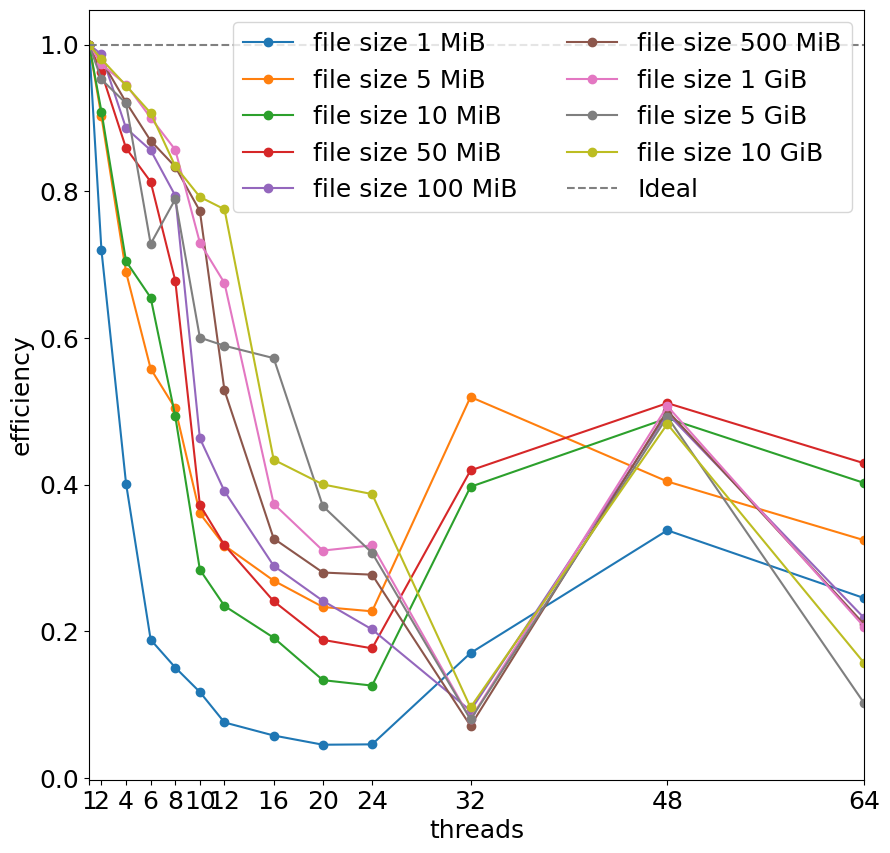
\includegraphics[width=\textwidth]{imgs/decode efficiency.png}
                \caption{Decoding efficiency}
                \label{fig:encoding-efficiency}
            \end{figure}
    \end{columns}
\end{frame}
\begin{frame}{Results - Barrier vs Locks}
    \begin{columns}
        \column{0.5\textwidth}
            \begin{figure}
                \centering
                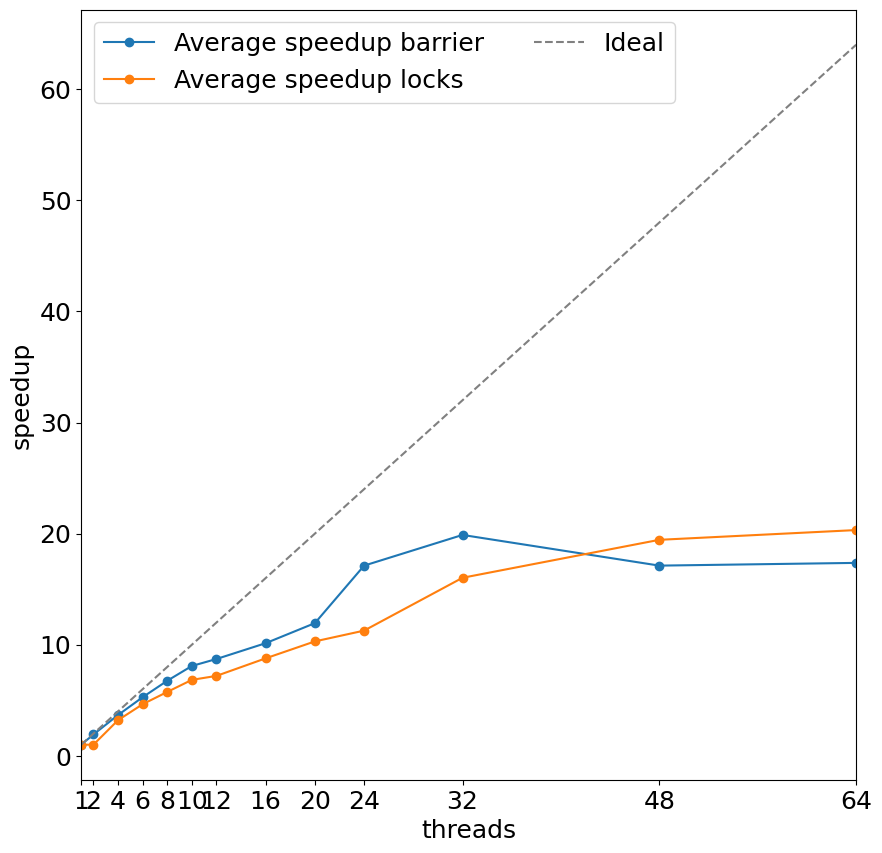
\includegraphics[width=\textwidth]{imgs/encode average speedup barrier vs locks.png}
                \caption{Encoding speedup barrier vs locks}
                \label{fig:encoding-speedup}
            \end{figure}
        \column{0.5\textwidth}
            \begin{figure}
                \centering
                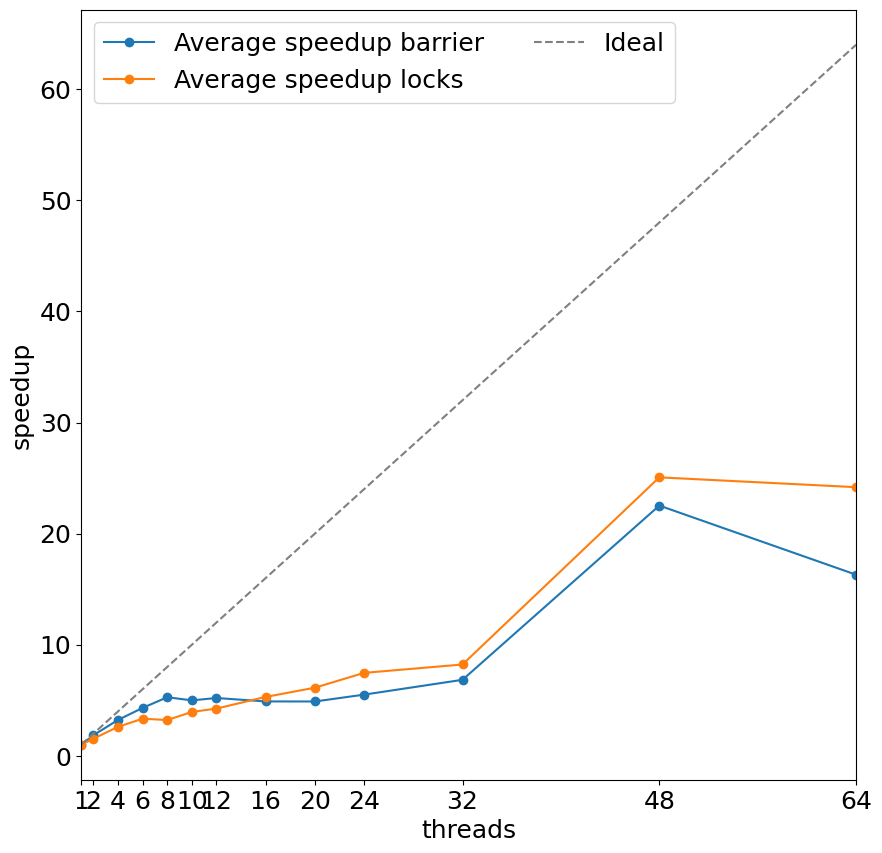
\includegraphics[width=\textwidth]{imgs/decode average speedup barrier vs locks}
                \caption{Decoding speedup barrier vs locks}
                \label{fig:encoding-efficiency}
            \end{figure}
    \end{columns}
\end{frame}
\begin{frame}{Results - Ours vs Online Implementation}
    \begin{columns}
        \column{0.5\textwidth}
            \begin{figure}
                \centering
                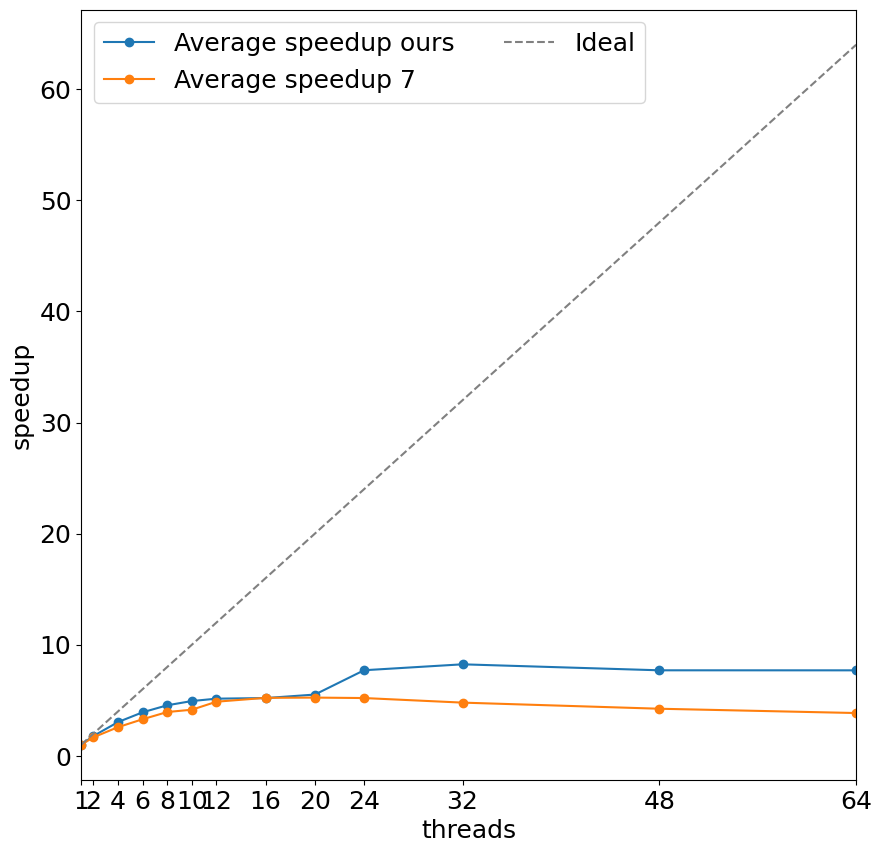
\includegraphics[width=\textwidth]{imgs/average ours vs 7}
                \caption{Average encoding speedup ours vs online 7}
                \label{fig:encoding-speedup}
            \end{figure}
        \column{0.5\textwidth}
            \begin{figure}
                \centering
                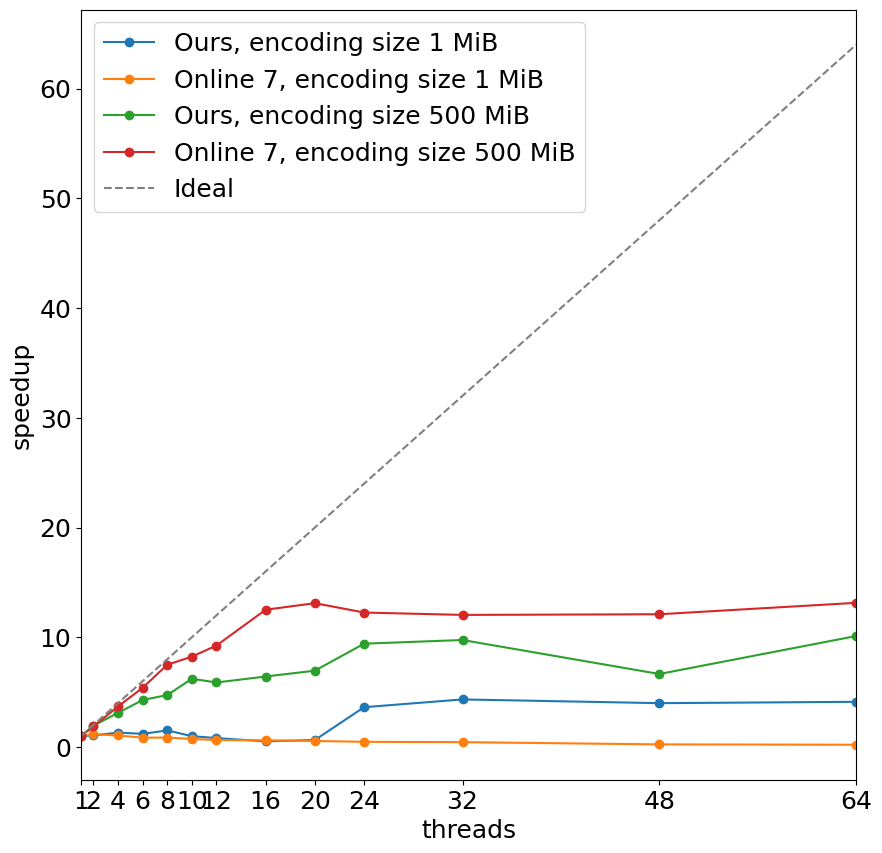
\includegraphics[width=\textwidth]{imgs/ours vs online 7 1-500}
                \caption{Encoding speedup ours vs online 7}
                \label{fig:encoding-efficiency}
            \end{figure}
    \end{columns}
\end{frame}
\begin{frame}{Results - Folders}

        \begin{figure}
            \centering
            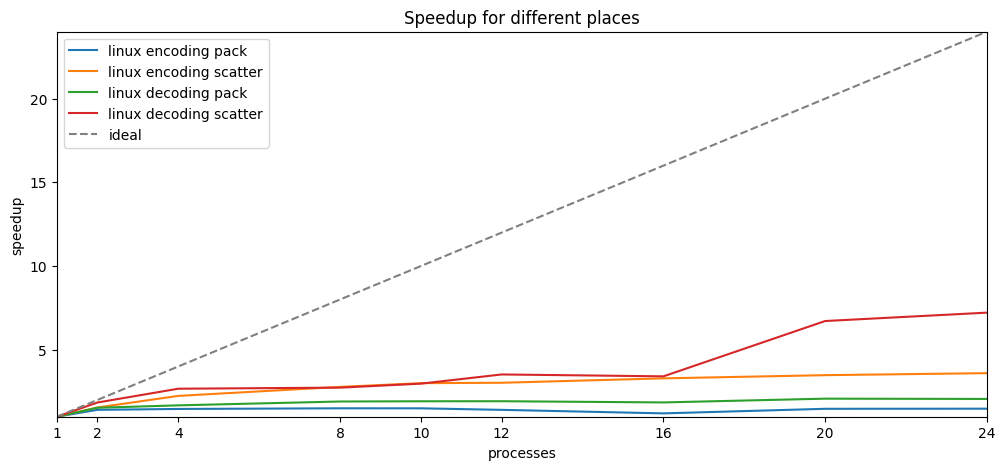
\includegraphics[width=\textwidth]{imgs/linux speedup.png}
            \caption{Encoding speedup with Linux}
            \label{fig:encoding-linux}
        \end{figure}
\end{frame}


% \include{sections/end.tex}
% \onecolumn
\pagebreak
\section{Appendix}

\subsection{Encoding}
\begin{table}[!h]
	\caption{Overall encoding times}
	\begin{tabular}{lrrrrrrrrrr}
		\toprule
		\diagbox{File sizes }{Threads} &        1  &        2  &        4  &        6  &        8  &        10 &       12 &        16 &       20 &       24 \\
		\midrule
		1 MiB   &    0.1084 &    0.1029 &    0.0826 &    0.0905 &    0.0718 &    0.1100 &   0.1338 &    0.2110 &   0.1705 &   0.2531 \\
		5 MiB   &    0.4073 &    0.2008 &    0.1255 &    0.1037 &    0.0970 &    0.0786 &   0.0789 &    0.0767 &   0.0906 &   0.0883 \\
		10 MiB  &    0.7611 &    0.4737 &    0.2658 &    0.2084 &    0.1804 &    0.1861 &   0.2204 &    0.3353 &   0.2432 &   0.3930 \\
		50 MiB  &    3.9241 &    2.1378 &    1.2788 &    1.0203 &    0.8575 &    0.7589 &   0.7773 &    0.6583 &   0.7523 &   0.9954 \\
		100 MiB &    7.7270 &    4.0680 &    2.4028 &    1.8596 &    1.5545 &    1.4324 &   1.2994 &    1.2468 &   1.2308 &   1.5375 \\
		500 MiB &   35.7753 &   18.3831 &   11.4959 &    8.3511 &    7.5589 &    5.7548 &   6.0857 &    5.5698 &   5.1431 &   5.0972 \\
		1 GiB   &   73.1120 &   38.1679 &   22.5066 &   16.3364 &   14.2131 &   13.7565 &  12.6196 &   10.8261 &  10.3345 &   9.7426 \\
		5 GiB   &  359.8495 &  186.6294 &   99.8038 &   77.4620 &   65.6555 &   67.3056 &  52.9090 &   48.4594 &  48.0126 &  48.8973 \\
		10 GiB  &  694.9750 &  370.5490 &  188.2278 &  136.1719 &  113.5878 &  104.0254 &  93.7227 &  116.8249 &  83.2084 &  82.0529 \\
		\bottomrule
	\end{tabular}
\end{table}
\begin{table}[!h]
	\caption{Pure encoding times}
	\begin{tabular}{lrrrrrrrrrr}
		\toprule
		\diagbox{File sizes }{Threads}  &        1  &        2  &        4  &        6  &       8  &       10 &       12 &       16 &       20 &       24 \\
		\midrule
		1 MiB   &    0.0637 &    0.0338 &    0.0184 &    0.0128 &   0.0100 &   0.0085 &   0.0388 &   0.0938 &   0.0351 &   0.1032 \\
		5 MiB   &    0.2980 &    0.1522 &    0.0782 &    0.0537 &   0.0413 &   0.0341 &   0.0296 &   0.0243 &   0.0207 &   0.0264 \\
		10 MiB  &    0.6547 &    0.3523 &    0.1845 &    0.1254 &   0.0977 &   0.0812 &   0.0730 &   0.1533 &   0.0570 &   0.1505 \\
		50 MiB  &    3.3027 &    1.7545 &    0.9147 &    0.6244 &   0.4884 &   0.4326 &   0.3432 &   0.2658 &   0.2953 &   0.3141 \\
		100 MiB &    6.7211 &    3.4461 &    1.8267 &    1.2448 &   0.9903 &   0.8153 &   0.6873 &   0.5415 &   0.4856 &   0.6148 \\
		500 MiB &   32.3825 &   16.6046 &    8.6817 &    6.2457 &   4.8624 &   4.0588 &   3.4132 &   2.6616 &   2.3853 &   2.0639 \\
		1 GiB   &   67.1756 &   34.0970 &   17.7353 &   12.6548 &   9.8790 &   8.2365 &   7.0042 &   5.4307 &   4.8915 &   4.2098 \\
		5 GiB   &  331.2526 &  174.0889 &   90.5618 &   63.4905 &  48.6453 &  38.9458 &  33.1852 &  26.1005 &  23.6226 &  20.4274 \\
		10 GiB  &  639.3369 &  328.5801 &  170.4086 &  119.6824 &  95.1232 &  79.8054 &  68.8753 &  53.3415 &  47.5727 &  48.6436 \\
		\bottomrule
	\end{tabular}
\end{table}
\begin{table}[!h]
	\caption{Overall encoding efficiency}
	\begin{tabular}{lrrrrrrrrrr}
		\toprule
		\diagbox{File sizes }{Threads} &   1  &      2  &      4  &      6  &      8  &      10 &      12 &      16 &      20 &      24 \\
		\midrule
		1 MiB   &  1.0 &  0.5272 &  0.3283 &  0.1997 &  0.1889 &  0.0986 &  0.0676 &  0.0321 &  0.0318 &  0.0179 \\
		5 MiB   &  1.0 &  1.0144 &  0.8111 &  0.6544 &  0.5250 &  0.5182 &  0.4302 &  0.3317 &  0.2247 &  0.1922 \\
		10 MiB  &  1.0 &  0.8034 &  0.7158 &  0.6086 &  0.5273 &  0.4090 &  0.2878 &  0.1419 &  0.1565 &  0.0807 \\
		50 MiB  &  1.0 &  0.9178 &  0.7671 &  0.6410 &  0.5721 &  0.5171 &  0.4207 &  0.3726 &  0.2608 &  0.1643 \\
		100 MiB &  1.0 &  0.9497 &  0.8040 &  0.6925 &  0.6213 &  0.5394 &  0.4956 &  0.3873 &  0.3139 &  0.2094 \\
		500 MiB &  1.0 &  0.9731 &  0.7780 &  0.7140 &  0.5916 &  0.6217 &  0.4899 &  0.4014 &  0.3478 &  0.2924 \\
		1 GiB   &  1.0 &  0.9578 &  0.8121 &  0.7459 &  0.6430 &  0.5315 &  0.4828 &  0.4221 &  0.3537 &  0.3127 \\
		5 GiB   &  1.0 &  0.9641 &  0.9014 &  0.7742 &  0.6851 &  0.5346 &  0.5668 &  0.4641 &  0.3747 &  0.3066 \\
		10 GiB  &  1.0 &  0.9378 &  0.9231 &  0.8506 &  0.7648 &  0.6681 &  0.6179 &  0.3718 &  0.4176 &  0.3529 \\
		\bottomrule
	\end{tabular}
\end{table}
\begin{table}[!h]
	\caption{Pure encoding efficiency}
	\begin{tabular}{lrrrrrrrrrr}
		\toprule
		\diagbox{File sizes }{Threads} &   1  &      2  &      4  &      6  &      8  &      10 &      12 &      16 &      20 &      24 \\
		\midrule
		1 MiB   &  1.0 &  0.9432 &  0.8677 &  0.8304 &  0.7960 &  0.7472 &  0.1370 &  0.0424 &  0.0908 &  0.0257 \\
		5 MiB   &  1.0 &  0.9788 &  0.9521 &  0.9253 &  0.9025 &  0.8729 &  0.8402 &  0.7654 &  0.7194 &  0.4697 \\
		10 MiB  &  1.0 &  0.9290 &  0.8872 &  0.8703 &  0.8373 &  0.8061 &  0.7476 &  0.2668 &  0.5743 &  0.1813 \\
		50 MiB  &  1.0 &  0.9412 &  0.9027 &  0.8816 &  0.8454 &  0.7635 &  0.8021 &  0.7767 &  0.5593 &  0.4381 \\
		100 MiB &  1.0 &  0.9752 &  0.9198 &  0.8999 &  0.8484 &  0.8244 &  0.8149 &  0.7757 &  0.6920 &  0.4555 \\
		500 MiB &  1.0 &  0.9751 &  0.9325 &  0.8641 &  0.8325 &  0.7978 &  0.7906 &  0.7604 &  0.6788 &  0.6538 \\
		1 GiB   &  1.0 &  0.9851 &  0.9469 &  0.8847 &  0.8500 &  0.8156 &  0.7992 &  0.7731 &  0.6867 &  0.6649 \\
		5 GiB   &  1.0 &  0.9514 &  0.9144 &  0.8696 &  0.8512 &  0.8505 &  0.8318 &  0.7932 &  0.7011 &  0.6757 \\
		10 GiB  &  1.0 &  0.9729 &  0.9379 &  0.8903 &  0.8401 &  0.8011 &  0.7735 &  0.7491 &  0.6720 &  0.5476 \\
		\bottomrule
	\end{tabular}
\end{table}
\pagebreak
\subsection{Encoding with Locks}
\begin{centering}
\begin{table}[!h]
	\caption{Overall encoding times}
	\begin{tabular}{rrrrrrrrrrrrrr}
		\toprule
		\diagbox[width=7em]{Size}{Threads} & 1  &      2  &      4  &      6  &      8  &      10 &     12 &     16 &     20 &     24 &     32 &     48 &     64 \\
		\midrule
		1 MiB   &   0.088 &   0.084 &   0.073 &   0.065 &   0.072 &   0.072 &  0.067 &  0.067 &  0.075 &  0.071 &  0.031 &  \textbf{0.027} &  0.033 \\
		5 MiB   &   0.425 &   0.406 &   0.275 &   0.172 &   0.167 &   0.164 &  0.148 &  0.139 &  0.139 &  0.136 &  \textbf{0.058} &  0.064 &  0.059 \\
		10 MiB  &   0.713 &   0.678 &   0.242 &   0.194 &   0.176 &   0.147 &  0.168 &  0.129 &  0.140 &  0.157 &  0.102 &  \textbf{0.094} &  0.102 \\
		50 MiB  &   3.585 &   3.371 &   1.141 &   0.838 &   0.748 &   0.698 &  0.961 &  0.968 &  0.733 &  0.895 &  0.430 &  \textbf{0.388} &  0.573 \\
		100 MiB &   6.805 &   6.601 &   2.159 &   1.622 &   1.359 &   1.200 &  1.098 &  0.974 &  0.888 &  0.842 &  0.771 &  \textbf{0.722} &  0.735 \\
		500 MiB &  33.464 &  31.995 &  10.564 &   7.854 &   6.683 &   6.041 &  5.518 &  5.931 &  4.577 &  4.248 &  4.140 &  \textbf{3.551} &  3.811 \\
		1 GiB   &  68.489 &  65.942 &  21.173 &  16.425 &  13.648 &  12.077 & 10.966 &  9.795 &  9.036 &  8.342 &  8.007 &  8.001 &  \textbf{7.69}0 \\
		5 GiB   & 367.228 & 370.850 & 110.299 &  84.128 &  75.319 &  66.408 & 59.666 & 59.479 & 51.181 & 48.904 & 38.824 & \textbf{38.677} & 40.676 \\
		10 GiB  & 676.529 & 642.922 & 187.620 & 135.991 & 123.822 & 109.770 & 96.643 & 93.226 & 90.825 & 88.154 & 63.886 & \textbf{61.847} & 64.598 \\
		\bottomrule
	\end{tabular}
	
\end{table}
\begin{table}[!h]
	\caption{Pure encoding times}
	\begin{tabular}{rrrrrrrrrrrrrr}
		\toprule
		\diagbox[width=7em]{Size}{Threads}  &      1  &      2  &      4  &      6  &     8  &     10 &     12 &     16 &     20 &     24 &     32 &     48 &     64 \\
		\midrule
		1 MiB   &   0.061 &   0.062 &   0.036 &   0.028 &  0.030 &  0.022 &  0.024 &  0.024 &  0.030 &  0.016 &  0.011 &  \textbf{0.009} &  0.011 \\
		5 MiB   &   0.361 &   0.363 &   0.209 &   0.109 &  0.103 &  0.092 &  0.079 &  0.066 &  0.053 &  0.050 &  0.023 &  0.023 &  \textbf{0.017} \\
		10 MiB  &   0.617 &   0.607 &   0.169 &   0.117 &  0.090 &  0.076 &  0.078 &  0.054 &  0.053 &  0.059 &  \textbf{0.03}9 &  \textbf{0.03}0 &  \textbf{0.03}5 \\
		50 MiB  &   3.131 &   3.057 &   0.847 &   0.595 &  0.464 &  0.416 &  0.671 &  0.652 &  0.435 &  0.500 &  0.186 &  \textbf{0.145} &  0.160 \\
		100 MiB &   6.079 &   6.037 &   1.664 &   1.151 &  0.891 &  0.735 &  0.642 &  0.521 &  0.438 &  0.386 &  0.327 &  0.285 &  \textbf{0.249} \\
		500 MiB &  31.001 &  30.471 &   8.287 &   5.810 &  4.519 &  3.778 &  3.226 &  2.610 &  2.227 &  1.946 &  1.814 &  1.430 &  \textbf{1.404} \\
		1 GiB   &  62.748 &  62.355 &  17.230 &  11.939 &  9.153 &  7.582 &  6.505 &  5.363 &  4.612 &  4.101 &  3.698 &  2.966 &  \textbf{2.833} \\
		5 GiB   & 343.876 & 351.067 &  99.909 &  73.825 & 62.694 & 54.050 & 47.849 & 42.794 & 33.944 & 29.952 & 18.749 & 14.847 & \textbf{14.376} \\
		10 GiB  & 629.449 & 623.710 & 172.829 & 120.552 & 94.623 & 78.728 & 68.025 & 55.215 & 46.723 & 41.474 & 32.493 & 27.176 & \textbf{23.935} \\
		\bottomrule
	\end{tabular}
\end{table}
\begin{table}[!h]
	\caption{Overall encoding efficiency}
	\begin{tabular}{rrrrrrrrrrrrrr}
		\toprule
		\diagbox[width=7em]{Size}{Threads}&    1  &    2  &    4  &    6  &    8  &    10 &    12 &    16 &    20 &    24 &    32 &    48 &    64 \\
		\midrule
		1 MiB   & 1.000 & 0.526 & 0.300 & 0.224 & 0.152 & 0.122 & 0.109 & 0.082 & 0.059 & 0.051 & 0.089 & 0.067 & 0.042 \\
		5 MiB   & 1.000 & 0.523 & 0.386 & 0.410 & 0.317 & 0.259 & 0.239 & 0.191 & 0.153 & 0.130 & 0.229 & 0.138 & 0.113 \\
		10 MiB  & 1.000 & 0.525 & 0.737 & 0.613 & 0.506 & 0.485 & 0.354 & 0.346 & 0.254 & 0.189 & 0.219 & 0.158 & 0.109 \\
		50 MiB  & 1.000 & 0.532 & 0.786 & 0.713 & 0.599 & 0.513 & 0.311 & 0.231 & 0.245 & 0.167 & 0.261 & 0.192 & 0.098 \\
		100 MiB & 1.000 & 0.515 & 0.788 & 0.699 & 0.626 & 0.567 & 0.516 & 0.437 & 0.383 & 0.337 & 0.276 & 0.196 & 0.145 \\
		500 MiB & 1.000 & 0.523 & 0.792 & 0.710 & 0.626 & 0.554 & 0.505 & 0.353 & 0.366 & 0.328 & 0.253 & 0.196 & 0.137 \\
		1 GiB   & 1.000 & 0.519 & 0.809 & 0.695 & 0.627 & 0.567 & 0.520 & 0.437 & 0.379 & 0.342 & 0.267 & 0.178 & 0.139 \\
		5 GiB   & 1.000 & 0.495 & 0.832 & 0.728 & 0.609 & 0.553 & 0.513 & 0.386 & 0.359 & 0.313 & 0.296 & 0.198 & 0.141 \\
		10 GiB  & 1.000 & 0.526 & 0.901 & 0.829 & 0.683 & 0.616 & 0.583 & 0.454 & 0.372 & 0.320 & 0.331 & 0.228 & 0.164 \\
		\bottomrule
	\end{tabular}
\end{table}
\begin{table}[!h]
	\caption{Pure encoding efficiency}
	\begin{tabular}{rrrrrrrrrrrrrr}
		\toprule
		\diagbox[width=7em]{Size}{Threads} &    1  &    2  &    4  &    6  &    8  &    10 &    12 &    16 &    20 &    24 &    32 &    48 &    64 \\
		\midrule
		1 MiB   & 1.000 & 0.493 & 0.425 & 0.367 & 0.252 & 0.283 & 0.209 & 0.160 & 0.101 & 0.161 & 0.172 & 0.138 & 0.085 \\
		5 MiB   & 1.000 & 0.497 & 0.431 & 0.551 & 0.438 & 0.391 & 0.380 & 0.344 & 0.341 & 0.300 & 0.491 & 0.331 & 0.334 \\
		10 MiB  & 1.000 & 0.508 & 0.913 & 0.881 & 0.852 & 0.816 & 0.655 & 0.714 & 0.583 & 0.436 & 0.495 & 0.426 & 0.275 \\
		50 MiB  & 1.000 & 0.512 & 0.924 & 0.878 & 0.843 & 0.753 & 0.389 & 0.300 & 0.360 & 0.261 & 0.525 & 0.449 & 0.306 \\
		100 MiB & 1.000 & 0.503 & 0.914 & 0.880 & 0.853 & 0.827 & 0.789 & 0.729 & 0.693 & 0.656 & 0.581 & 0.444 & 0.381 \\
		500 MiB & 1.000 & 0.509 & 0.935 & 0.889 & 0.857 & 0.821 & 0.801 & 0.742 & 0.696 & 0.664 & 0.534 & 0.452 & 0.345 \\
		1 GiB   & 1.000 & 0.503 & 0.910 & 0.876 & 0.857 & 0.828 & 0.804 & 0.731 & 0.680 & 0.638 & 0.530 & 0.441 & 0.346 \\
		5 GiB   & 1.000 & 0.490 & 0.860 & 0.776 & 0.686 & 0.636 & 0.599 & 0.502 & 0.507 & 0.478 & 0.573 & 0.483 & 0.374 \\
		10 GiB  & 1.000 & 0.505 & 0.911 & 0.870 & 0.832 & 0.800 & 0.771 & 0.712 & 0.674 & 0.632 & 0.605 & 0.483 & 0.411 \\
		\bottomrule
	\end{tabular}
\end{table}
\end{centering}
\pagebreak
\subsection{Decoding}
\begin{centering}
\begin{table}[!h]
	\caption{Overall decoding times}
	\begin{tabular}{rrrrrrrrrrrrrr}
		\toprule
		\diagbox[width=7em]{Size}{Threads} &      1  &      2  &      4  &      6  &      8  &      10 &      12 &      16 &      20 &      24 &      32 &      48 &      64 \\
		\midrule
		1 MiB   &   0.130 &   0.091 &   0.079 &   0.099 &   0.091 &   0.097 &   0.118 &   0.115 &   0.119 &   0.104 &   0.045 &   \textbf{0.026} &   0.030 \\
		5 MiB   &   0.422 &   0.253 &   0.177 &   0.166 &   0.141 &   0.156 &   0.151 &   0.139 &   0.130 &   0.121 &   0.087 &   0.087 &   \textbf{0.082} \\
		10 MiB  &   0.871 &   0.517 &   0.384 &   0.296 &   0.293 &   0.433 &   0.372 &   0.356 &   0.368 &   0.355 &   0.171 &   \textbf{0.129} &   0.161 \\
		50 MiB  &   4.108 &   2.277 &   1.511 &   1.252 &   1.276 &   1.382 &   1.412 &   1.409 &   1.434 &   1.328 &   0.693 &   0.594 &   \textbf{0.544} \\
		100 MiB &   7.961 &   4.507 &   2.915 &   2.275 &   1.884 &   2.418 &   2.400 &   2.422 &   2.343 &   2.251 &   4.392 &   1.858 &   \textbf{1.722} \\
		500 MiB &  37.619 &  22.511 &  13.501 &  11.334 &  10.035 &   9.326 &   9.640 &  11.182 &  11.069 &  10.021 &  19.667 &   \textbf{5.68}0 &   7.006 \\
		1 GiB   &  76.679 &  43.252 &  27.585 &  23.271 &  18.590 &  17.824 &  18.532 &  22.027 &  19.813 &  17.128 &  37.634 &  \textbf{12.183} &  14.964 \\
		5 GiB   & 361.871 & 193.112 & 108.812 &  96.790 &  81.066 &  84.897 &  79.142 &  \textbf{73.725} &  79.374 &  75.976 & 155.945 & 111.347 &  81.739 \\
		10 GiB  & 759.072 & 391.202 & 212.381 & 156.396 & 135.844 & 135.401 & 134.098 & 138.000 & 134.006 & 132.255 & 253.313 & \textbf{106.227} & 119.210 \\
		\bottomrule
	\end{tabular}
\end{table}

\begin{table}[!h]
	\caption{Pure decoding times}
	\begin{tabular}{rrrrrrrrrrrrrr}
		\toprule
		\diagbox[width=7em]{Size}{Threads} &      1  &      2  &      4  &      6  &      8  &     10 &     12 &      16 &     20 &     24 &      32 &     48 &     64 \\
		\midrule
		1 MiB   &   0.083 &   0.058 &   0.052 &   0.074 &   0.069 &  0.071 &  0.092 &   0.090 &  0.092 &  0.076 &   0.015 &  \textbf{0.005} &  \textbf{0.005} \\
		5 MiB   &   0.340 &   0.188 &   0.123 &   0.101 &   0.084 &  0.094 &  0.089 &   0.079 &  0.073 &  0.062 &   0.020 &  0.018 &  \textbf{0.016} \\
		10 MiB  &   0.752 &   0.414 &   0.267 &   0.191 &   0.191 &  0.265 &  0.267 &   0.246 &  0.282 &  0.249 &   0.059 &  0.032 &  \textbf{0.029} \\
		50 MiB  &   3.634 &   1.888 &   1.058 &   0.745 &   0.670 &  0.976 &  0.954 &   0.943 &  0.966 &  0.857 &   0.271 &  0.148 &  \textbf{0.132} \\
		100 MiB &   7.132 &   3.613 &   2.012 &   1.388 &   1.123 &  1.540 &  1.520 &   1.541 &  1.478 &  1.468 &   2.433 &  \textbf{0.299} &  0.511 \\
		500 MiB &  36.395 &  18.594 &   9.874 &   6.980 &   5.458 &  4.707 &  5.739 &   6.970 &  6.499 &  5.473 &  16.056 &  \textbf{1.514} &  2.716 \\
		1 GiB   &  74.764 &  38.408 &  19.764 &  13.840 &  10.908 & 10.242 &  9.231 &  12.504 & 12.060 &  9.825 &  29.059 &  \textbf{3.072} &  5.671 \\
		5 GiB   & 359.883 & 188.886 &  97.788 &  82.355 &  56.999 & 59.936 & 50.887 &  39.291 & 48.562 & 48.877 & 141.437 & \textbf{15.227} & 55.262 \\
		10 GiB  & 754.842 & 385.021 & 199.850 & 138.739 & 113.105 & 95.262 & 81.112 & 108.727 & 94.317 & 81.262 & 245.681 & \textbf{32.584} & 75.318 \\
		\bottomrule
	\end{tabular}
\end{table}

\begin{table}[!h]
	\caption{Overall decoding efficiency}
	\begin{tabular}{rrrrrrrrrrrrrr}
		\toprule
		\diagbox[width=7em]{Size}{Threads}  &    1  &    2  &    4  &    6  &    8  &    10 &    12 &    16 &    20 &    24 &    32 &    48 &    64 \\
		\midrule
		1 MiB   & 1.000 & 0.719 & 0.411 & 0.220 & 0.179 & 0.134 & 0.092 & 0.071 & 0.055 & 0.052 & 0.090 & 0.103 & 0.067 \\
		5 MiB   & 1.000 & 0.835 & 0.595 & 0.423 & 0.374 & 0.270 & 0.233 & 0.189 & 0.163 & 0.145 & 0.152 & 0.101 & 0.080 \\
		10 MiB  & 1.000 & 0.842 & 0.567 & 0.491 & 0.371 & 0.201 & 0.195 & 0.153 & 0.118 & 0.102 & 0.159 & 0.140 & 0.085 \\
		50 MiB  & 1.000 & 0.902 & 0.680 & 0.547 & 0.402 & 0.297 & 0.242 & 0.182 & 0.143 & 0.129 & 0.185 & 0.144 & 0.118 \\
		100 MiB & 1.000 & 0.883 & 0.683 & 0.583 & 0.528 & 0.329 & 0.276 & 0.205 & 0.170 & 0.147 & 0.057 & 0.089 & 0.072 \\
		500 MiB & 1.000 & 0.836 & 0.697 & 0.553 & 0.469 & 0.403 & 0.325 & 0.210 & 0.170 & 0.156 & 0.060 & 0.138 & 0.084 \\
		1 GiB   & 1.000 & 0.886 & 0.695 & 0.549 & 0.516 & 0.430 & 0.345 & 0.218 & 0.194 & 0.187 & 0.064 & 0.131 & 0.080 \\
		5 GiB   & 1.000 & 0.937 & 0.831 & 0.623 & 0.558 & 0.426 & 0.381 & 0.307 & 0.228 & 0.198 & 0.073 & 0.068 & 0.069 \\
		10 GiB  & 1.000 & 0.970 & 0.894 & 0.809 & 0.698 & 0.561 & 0.472 & 0.344 & 0.283 & 0.239 & 0.094 & 0.149 & 0.099 \\
		\bottomrule
	\end{tabular}
\end{table}

\begin{table}[!h]
	\caption{Pure decoding efficiency}
	\begin{tabular}{rrrrrrrrrrrrrr}
		\toprule
		\diagbox[width=7em]{Size}{Threads} &    1  &    2  &    4  &    6  &    8  &    10 &    12 &    16 &    20 &    24 &    32 &    48 &    64 \\
		\midrule
		1 MiB   & 1.000 & 0.720 & 0.401 & 0.188 & 0.150 & 0.117 & 0.075 & 0.058 & 0.045 & 0.046 & 0.170 & 0.338 & 0.245 \\
		5 MiB   & 1.000 & 0.902 & 0.690 & 0.558 & 0.504 & 0.361 & 0.317 & 0.269 & 0.233 & 0.227 & 0.519 & 0.404 & 0.324 \\
		10 MiB  & 1.000 & 0.909 & 0.705 & 0.655 & 0.493 & 0.284 & 0.234 & 0.191 & 0.133 & 0.126 & 0.397 & 0.490 & 0.402 \\
		50 MiB  & 1.000 & 0.962 & 0.859 & 0.813 & 0.678 & 0.372 & 0.317 & 0.241 & 0.188 & 0.177 & 0.419 & 0.511 & 0.429 \\
		100 MiB & 1.000 & 0.987 & 0.886 & 0.856 & 0.794 & 0.463 & 0.391 & 0.289 & 0.241 & 0.202 & 0.092 & 0.497 & 0.218 \\
		500 MiB & 1.000 & 0.979 & 0.922 & 0.869 & 0.834 & 0.773 & 0.528 & 0.326 & 0.280 & 0.277 & 0.071 & 0.501 & 0.209 \\
		1 GiB   & 1.000 & 0.973 & 0.946 & 0.900 & 0.857 & 0.730 & 0.675 & 0.374 & 0.310 & 0.317 & 0.080 & 0.507 & 0.206 \\
		5 GiB   & 1.000 & 0.953 & 0.920 & 0.728 & 0.789 & 0.600 & 0.589 & 0.572 & 0.371 & 0.307 & 0.080 & 0.492 & 0.102 \\
		10 GiB  & 1.000 & 0.980 & 0.944 & 0.907 & 0.834 & 0.792 & 0.776 & 0.434 & 0.400 & 0.387 & 0.096 & 0.483 & 0.157 \\
		\bottomrule
	\end{tabular}
\end{table}
\end{centering}

\pagebreak
\subsection{Decoding with Locks}
\begin{centering}
\begin{table}[!h]
	\caption{Overall decoding times}
	\begin{tabular}{lrrrrrrrrrrrrr}
		\toprule
		\diagbox[width=7em]{Sizes}{Threads}  & 1  &      2  &      4  &      6  &      8  &      10 &      12 &      16 &      20 &      24 &      32 &      48 &      64 \\
		\midrule
		1 MiB   &   0.272 &   0.212 &   0.116 &   0.101 &   0.070 &   0.068 &   0.066 &   0.069 &   0.075 &   0.093 &   0.095 &   \textbf{0.036} &   \textbf{0.036} \\
		5 MiB   &   0.635 &   0.915 &   1.265 &   0.655 &   0.684 &   0.289 &   0.482 &   0.298 &   0.330 &   0.180 &   0.562 &   \textbf{0.124} &   0.254 \\
		10 MiB  &   0.861 &   0.501 &   0.333 &   0.271 &   0.269 &   0.258 &   0.236 &   0.217 &   0.190 &   \textbf{0.183} &   0.604 &   0.440 &   0.404 \\
		50 MiB  &   3.991 &   2.248 &   1.462 &   1.176 &   1.160 &   1.088 &   1.017 &   0.913 &   0.837 &   0.775 &   1.409 &   0.761 &   \textbf{0.726} \\
		100 MiB &   7.615 &  33.645 &  15.250 &  11.628 &  13.018 &  10.761 &   9.192 &   3.661 &   5.691 &   4.475 &   2.175 &   \textbf{1.312} &   1.464 \\
		500 MiB &  37.082 &  20.422 &  13.236 &  11.344 &  10.774 &  10.441 &   9.767 &   8.661 &   7.387 &   7.051 &  10.581 &   9.984 &   \textbf{6.591} \\
		1 GiB   &  73.855 &  41.185 &  26.929 &  23.051 &  17.977 &  18.781 &  19.731 &  17.837 &  16.171 &  15.437 &  19.766 &  14.432 &  \textbf{12.636} \\
		5 GiB   & 352.386 & 475.087 & 265.894 & 204.661 & 156.227 & 139.894 & 127.649 & 109.245 & 100.918 &  89.890 & 104.173 &  65.082 &  \textbf{63.837} \\
		10 GiB  & 714.907 & 376.029 & 202.712 & 190.071 & 435.224 & 145.673 & 133.319 & 122.774 & 117.529 & \textbf{115.262} & 158.281 & 150.057 & 148.834 \\
		\bottomrule
	\end{tabular}
\end{table}

\begin{table}[!h]
	\caption{Pure decoding times}
	\begin{tabular}{lrrrrrrrrrrrrr}
		\toprule
		\diagbox[width=7em]{Sizes}{Threads} & 1  &      2  &      4  &      6  &      8  &      10 &      12 &     16 &     20 &     24 &      32 &     48 &     64 \\
		\midrule
		1 MiB   &   0.116 &   0.064 &   0.056 &   0.056 &   0.041 &   0.041 &   0.038 &  0.041 &  0.038 &  0.035 &   0.061 &  \textbf{0.006} &  0.007 \\
		5 MiB   &   0.565 &   0.859 &   1.202 &   0.598 &   0.627 &   0.234 &   0.425 &  0.244 &  0.269 &  0.113 &   0.019 &  0.017 &  \textbf{0.016} \\
		10 MiB  &   0.715 &   0.399 &   0.234 &   0.174 &   0.169 &   0.159 &   0.136 &  0.119 &  0.095 &  0.085 &   0.132 &  0.031 &  \textbf{0.028} \\
		50 MiB  &   3.531 &   1.848 &   1.034 &   0.742 &   0.730 &   0.656 &   0.620 &  0.486 &  0.417 &  0.352 &   0.703 &  0.143 &  \textbf{0.117} \\
		100 MiB &   6.874 &  33.366 &  14.884 &  10.786 &  12.377 &   9.907 &   8.348 &  2.879 &  5.046 &  3.695 &   0.968 &  \textbf{0.285} &  0.510 \\
		500 MiB &  35.450 &  18.238 &  10.009 &   7.179 &   6.792 &   6.317 &   5.622 &  4.667 &  3.831 &  3.280 &   6.218 &  1.394 &  \textbf{1.212} \\
		1 GiB   &  72.114 &  36.926 &  20.113 &  14.503 &  11.600 &  12.692 &  11.302 &  9.281 &  7.654 &  6.478 &   9.440 &  2.841 &  \textbf{2.705} \\
		5 GiB   & 349.890 & 471.340 & 257.714 & 197.061 & 140.154 & 124.853 & 110.634 & 91.401 & 74.582 & 62.539 &  73.525 & 14.510 & \textbf{12.708} \\
		10 GiB  & 711.985 & 370.520 & 191.792 & 182.3175 & 421.918 & 126.678 & 113.482 & 92.082 & 76.309 & 64.483 & 100.849 & \textbf{29.389} & 54.947 \\
		\bottomrule
	\end{tabular}
\end{table}

\begin{table}[!h]
	\caption{Overall decoding efficiency}
	\begin{tabular}{lrrrrrrrrrrrrr}
		\toprule
		\diagbox[width=7em]{Sizes}{Threads} & 1  &    2  &    4  &    6  &    8  &    10 &    12 &    16 &    20 &    24 &    32 &    48 &    64 \\
		\midrule
		1 MiB   & 1.000 & 0.642 & 0.585 & 0.450 & 0.486 & 0.402 & 0.346 & 0.245 & 0.182 & 0.122 & 0.089 & 0.157 & 0.119 \\
		5 MiB   & 1.000 & 0.347 & 0.126 & 0.162 & 0.116 & 0.220 & 0.110 & 0.133 & 0.096 & 0.147 & 0.035 & 0.107 & 0.039 \\
		10 MiB  & 1.000 & 0.860 & 0.647 & 0.529 & 0.400 & 0.334 & 0.303 & 0.248 & 0.227 & 0.196 & 0.045 & 0.041 & 0.033 \\
		50 MiB  & 1.000 & 0.888 & 0.683 & 0.566 & 0.430 & 0.367 & 0.327 & 0.273 & 0.238 & 0.215 & 0.089 & 0.109 & 0.086 \\
		100 MiB & 1.000 & 0.113 & 0.125 & 0.109 & 0.073 & 0.071 & 0.069 & 0.130 & 0.067 & 0.071 & 0.109 & 0.121 & 0.081 \\
		500 MiB & 1.000 & 0.908 & 0.700 & 0.545 & 0.430 & 0.355 & 0.316 & 0.268 & 0.251 & 0.219 & 0.110 & 0.077 & 0.088 \\
		1 GiB   & 1.000 & 0.897 & 0.686 & 0.534 & 0.514 & 0.393 & 0.312 & 0.259 & 0.228 & 0.199 & 0.117 & 0.107 & 0.091 \\
		5 GiB   & 1.000 & 0.371 & 0.331 & 0.287 & 0.282 & 0.252 & 0.230 & 0.202 & 0.175 & 0.163 & 0.106 & 0.113 & 0.086 \\
		10 GiB  & 1.000 & 0.951 & 0.881 & 0.625 & 0.205 & 0.491 & 0.447 & 0.364 & 0.304 & 0.258 & 0.141 & 0.099 & 0.075 \\
		\bottomrule
	\end{tabular}
\end{table}

\begin{table}[!h]
	\caption{Pure decoding efficiency}
	\begin{tabular}{lrrrrrrrrrrrrr}
		\toprule
		\diagbox[width=7em]{Sizes}{Threads} & 1  &    2  &    4  &    6  &    8  &    10 &    12 &    16 &    20 &    24 &    32 &    48 &    64 \\
		\midrule
		1 MiB   & 1.000 & 0.901 & 0.515 & 0.349 & 0.357 & 0.285 & 0.255 & 0.176 & 0.152 & 0.138 & 0.060 & 0.428 & 0.260 \\
		5 MiB   & 1.000 & 0.329 & 0.118 & 0.157 & 0.113 & 0.242 & 0.111 & 0.145 & 0.105 & 0.208 & 0.918 & 0.703 & 0.551 \\
		10 MiB  & 1.000 & 0.897 & 0.764 & 0.684 & 0.529 & 0.449 & 0.437 & 0.376 & 0.377 & 0.351 & 0.169 & 0.486 & 0.402 \\
		50 MiB  & 1.000 & 0.955 & 0.854 & 0.793 & 0.605 & 0.538 & 0.474 & 0.454 & 0.423 & 0.418 & 0.157 & 0.516 & 0.471 \\
		100 MiB & 1.000 & 0.103 & 0.115 & 0.106 & 0.069 & 0.069 & 0.069 & 0.149 & 0.068 & 0.078 & 0.222 & 0.502 & 0.210 \\
		500 MiB & 1.000 & 0.972 & 0.885 & 0.823 & 0.652 & 0.561 & 0.525 & 0.475 & 0.463 & 0.450 & 0.178 & 0.530 & 0.457 \\
		1 GiB   & 1.000 & 0.976 & 0.896 & 0.829 & 0.777 & 0.568 & 0.532 & 0.486 & 0.471 & 0.464 & 0.239 & 0.529 & 0.417 \\
		5 GiB   & 1.000 & 0.371 & 0.339 & 0.296 & 0.312 & 0.280 & 0.264 & 0.239 & 0.235 & 0.233 & 0.149 & 0.502 & 0.430 \\
		10 GiB  & 1.000 & 0.9606 & 0.928 & 0.651 & 0.211 & 0.562 & 0.523 & 0.483 & 0.467 & 0.460 & 0.221 & 0.505 & 0.202 \\
		\bottomrule
	\end{tabular}
\end{table}
\end{centering}
\pagebreak
%\twocolumn
\input{sections/results/linux local}

% \begin{frame}{Column slide}
%     \begin{columns}
%         \column{0.50\textwidth}
%         column1

%         \column{0.50\textwidth}
%         column2
%     \end{columns}
% \end{frame}


% \begin{frame}{Block examples}
%     \begin{block}{Observation 1}
%         Simmons Hall is composed of metal and concrete.
%     \end{block}
%     \begin{exampleblock}{Observation 2}
%         Simmons Hall is composed of metal and concrete.
%     \end{exampleblock}
%     \begin{textbfblock}{Conclusion}
%         Simmons Hall $\not=$ Simmons Dormitory.
%     \end{textbfblock}
% \end{frame}
% \begin{frame}[allowframebreaks,noframenumbering]
% \frametitle{References}
%\bibliographystyle{amsalpha}
% \bibliographystyle{unsrt}
% \bibliography{../report/bibliography.bib}{}
% \end{frame}
\end{document}

